\chapter{\label{chapter4}Implementation}

In this chapter, we show how Swift was implemented into iSDX. We give an overview of the modified iSDX architecture in \ref{chapter4:Architecture}. We explain the two new modules that were added to the iSDX in \ref{chapter4:Swift-BPA} and in \ref{chapter4:FR-handler}, respectively. We explain the VMAC partitioning in \ref{chapter4:vmac_partitioning} and explain what was changed in the default iSDX modules in \ref{chapter4:Changes_to_the_iSDX}.

In the next chapter we present the results of the tests done to measure the convergence performance of the iSDX.

\section{\label{chapter4:Architecture}Architecture}

\begin{figure}[h]
\center
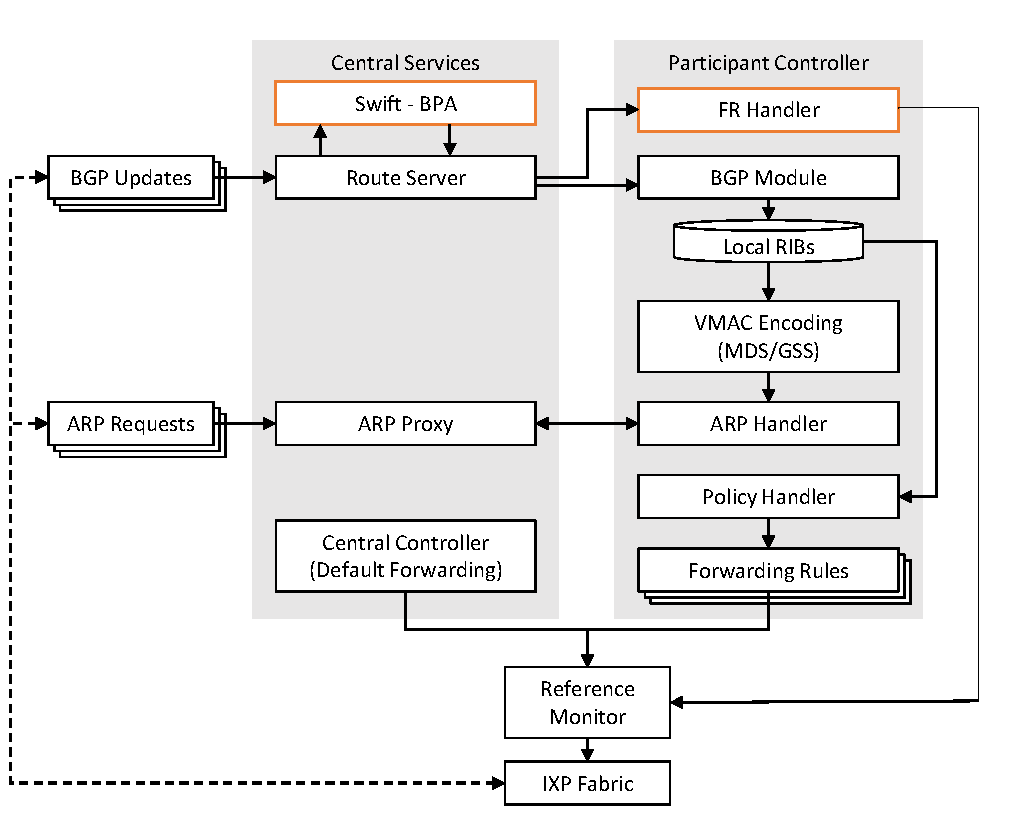
\includegraphics[scale = 0.7]{Figures/design_sdx_swift_cropped.pdf}
\caption{iSDX architecture with Swift}
\label{fig:isdx_architecture_with_swift}
\end{figure}

Figure~\ref{fig:isdx_architecture_with_swift} shows the iSDX~\cite{feamster2013sdx} architecture with Swift. The orange modules represent the new modules we had to add to the iSDX to implement Swift. The iSDX receives two additional modules the Swift-BPA module in the central services and the FR handler in the participant controller. With these two modules the iSDX will now detect bursts of withdrawals, predict the failed AS-link and push fast reroute rules into the IXP fabric. \\
In the following sections, I will go over the functionality of the new modules and other changes to the iSDX in more detail.

\section{\label{chapter4:Swift-BPA}Swift-BPA}

\begin{figure}[h]
\center
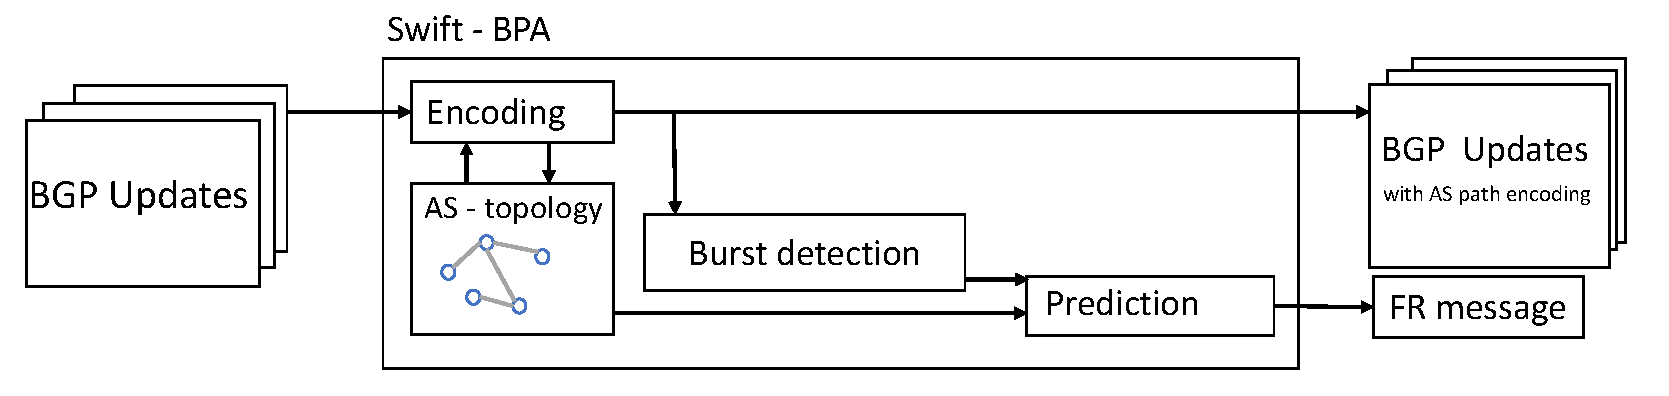
\includegraphics[scale = 0.5]{Figures/design_swift_bpa_cropped.pdf}
\caption{pipeline of the Swift-BPA module}
\end{figure}

The Swift-BPA module implements Swifts main functionality, encoding and prediction. It is part of the central services and exchanges BGP updates and FR messages with the route server and participant controllers.

The Swift-BPA module is placed at the route server and processes each update received by the route server before passing it on to the participant controllers. 
When receiving a BGP update the Swift-BPA updates the AS-topology and adds the AS-path encoding to the BGP update. Then the update gets sent to the participant controller. 
After the update is sent to the participant controller the burst detection checks if the update triggers a burst. If so the prediction module predicts the failed AS-link and sends FR messages to the participant controller. 
The fast reroute message informs the participant controllers about the AS-link that is predicted to be down. 

Similar to the participant controller every participant has a Swift-BPA process running. The Swift-BPA only receives BGP updates from his own routers. This way the Swift engine can be implemented without any modifications.

\section{\label{chapter4:FR-handler}FR-Handler}

\begin{figure}[h]
\center
\includegraphics[scale = 0.6]{Figures/design_fr_handler_cropped.pdf}
\caption{pipeline of the fast reroute handler}
\end{figure}

The FR-handler implements the pushing of fast reroute rules.  \\
Once the Swift-BPA predicts a failed AS-link it sends FR messages to all the participant \\ controllers.
The FR-handler receives FR messages and computes the fast reroute rules using the backup next-hops and the predicted AS-link. Every participant controller computes its own backup next-hops. \\ The fast reroute rules get sent to the reference monitor as flow rule messages. The reference monitor then installs the flow rules in the SDN switch. Just like in Swift the fast reroute rules match on the failed AS-link and on the backup next-hop.    

\newpage

\section{\label{chapter4:vmac_partitioning}VMAC Partitioning}

Both Swift and the iSDX use the destination mac address as a VMAC to attach additional information to the packet. It is not easy to use another field of the header as only the destination mac address can be changed by modifying the next hop attribute. Therefore the VMAC has to be shared between the iSDX and the Swift encoding. The number of bits available to encode information for the iSDX and Swift is reduced. This is because the iSDX and Swift encode \\ 
different information about the prefix. The iSDX encodes the participants advertising the prefix and the BGP best next hop. Swift encodes the AS-path and the backup next hops for each link on the AS-path.

The encoded AS-path starts with the second AS on the AS-path. This is because the first AS is already encoded as the BGP best next-hop. (in the iSDX part of the VMAC)

\begin{figure}[h]
\center
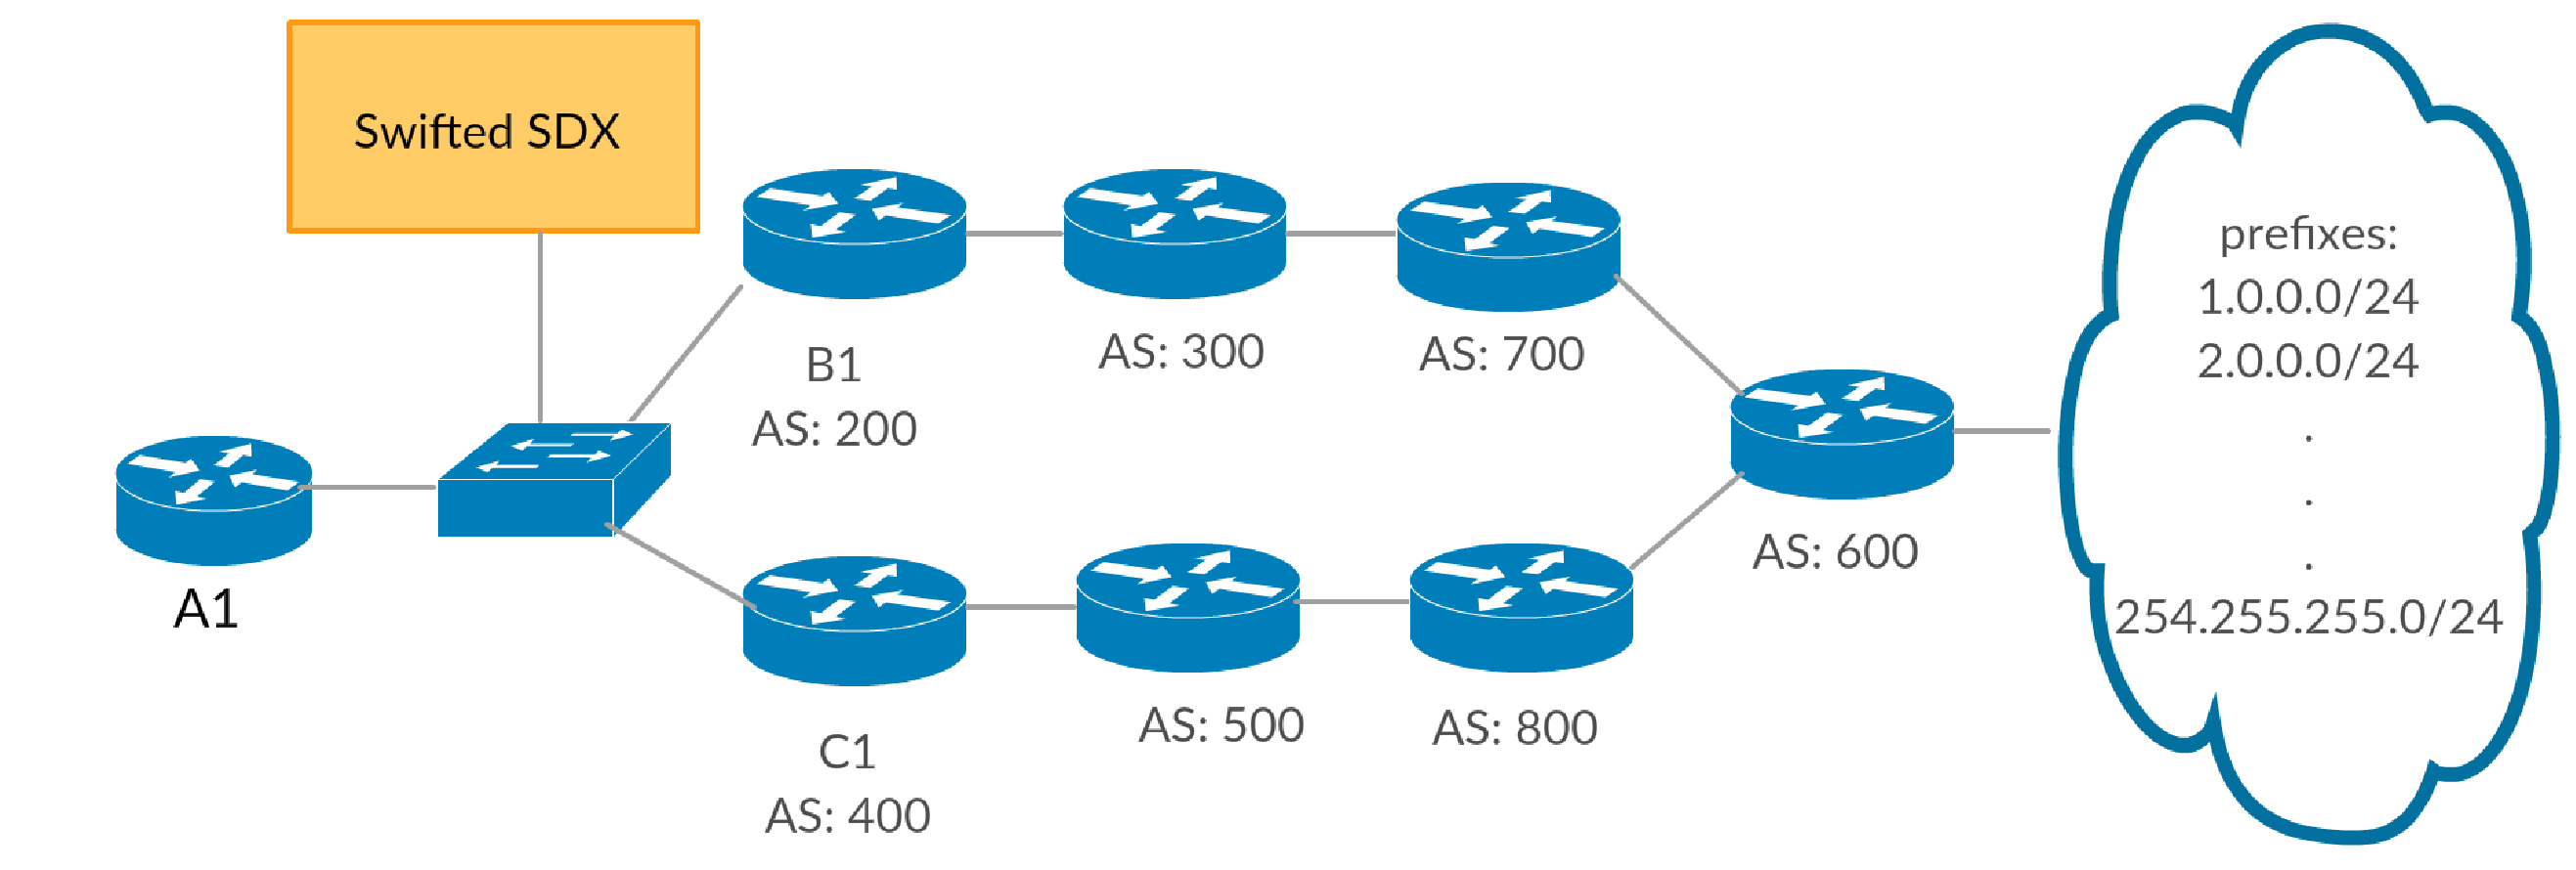
\includegraphics[scale = 0.24]{Figures/design_vmac_topology.pdf}
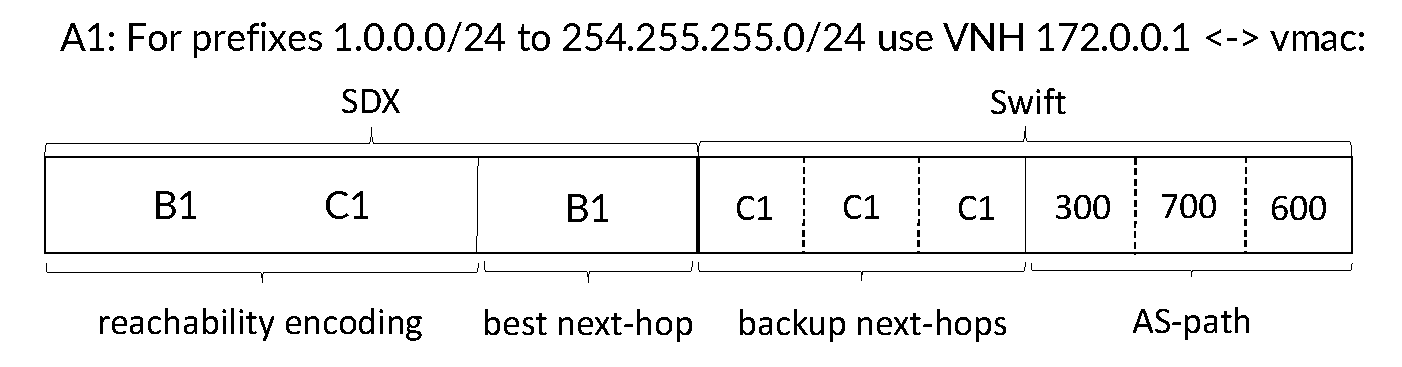
\includegraphics[scale = 0.35]{Figures/design_vmac_cropped.pdf}
\caption{example of the VMAC in the iSDX with Swift}
\end{figure}

\section{\label{chapter4:Changes_to_the_iSDX}Changes to the iSDX}

We also had to apply a few changes to the iSDX's modules. These changes mainly affect the route server, the local RIB of the participant controller and the VMAC encoding. 

\paragraph{\label{chapter4:Changes to the iSDX:route server}Route Server:}

The route server had to be adapted to work with the Swift-BPA module. 
The route server now has two modules the Listener and Sender. \\
The Listener receives BGP updates and forwards them to the Swift-BPA. \\
The Sender receives modified BGP updates and FR messages from the Swift-BPA and forwards them to the participant controllers. The sender processes FR messages with higher priority than modified BGP updates, this way the FR messages reach the FR handlers as quickly as possible. 

\begin{figure}[h]
\center
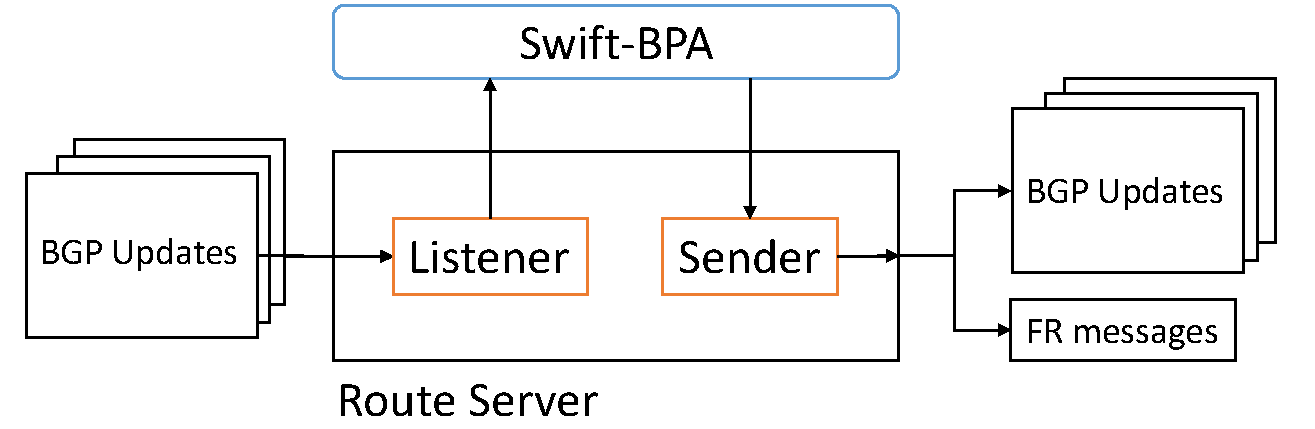
\includegraphics[scale = 0.45]{Figures/design_route_server_cropped2.pdf}
\caption{pipeline of the modified route server}
\end{figure}


\paragraph{\label{chapter4:Changes to the iSDX:local RIB}Local RIB:}

The local RIB now stores the AS-path encoding. When processing a BGP update the local RIB extracts the AS-path encoding (added by the Swift-BPA) and saves it as an additional attribute. The encoded AS-path is then used in the VMAC encoding. 

\paragraph{\label{chapter4:Changes to the iSDX:Vmac Encoding}VMAC Encoding:}
The VMAC encoding now computes the backup next-hops for the AS-path of the BGP update. There is one backup next-hop for every AS-link on the AS-path, packets can be sent to the backup next-hop in case this AS-link is predicted to be down. \\
The VMAC encoding now builds the VMAC using both iSDX and Swift encoding. \\

\newpage
